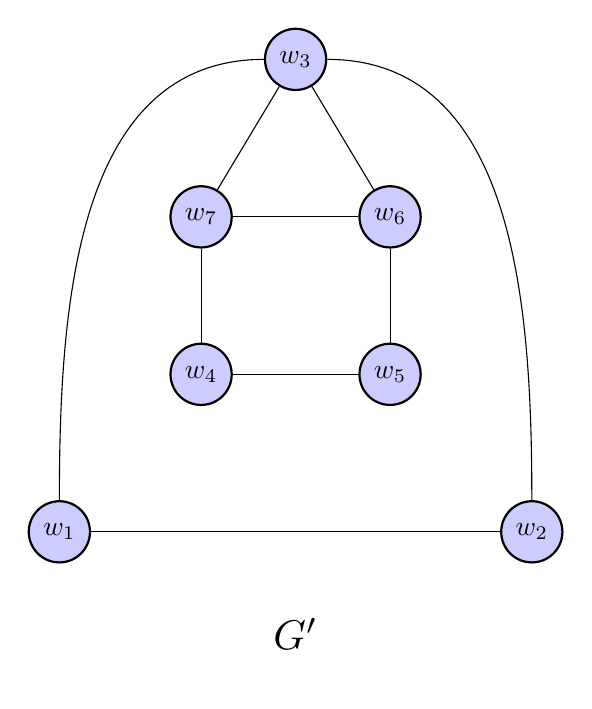
\begin{tikzpicture}[auto=left,every node/.style={circle,fill=blue!20,draw=black,thick}]
  % Vértice superior en la misma cota máxima (y=3.5)
  \node (w3) at (0, 3.5) {$w_3$};

  % "Casa" interior (w7, w6, w5, w4)
  \node (w7) at (-1.2, 1.5) {$w_7$};
  \node (w6) at (1.2, 1.5) {$w_6$};
  \node (w5) at (1.2, -0.5) {$w_5$};
  \node (w4) at (-1.2, -0.5) {$w_4$};

  % Vértices inferiores en la misma cota mínima (y=-2.5)
  \node (w1) at (-3, -2.5) {$w_1$};
  \node (w2) at (3, -2.5) {$w_2$};

  % Aristas de la estructura interior
  \foreach \from/\to in {w7/w6, w6/w5, w5/w4, w4/w7, w3/w7, w3/w6}
    \draw (\from) -- (\to);

  % Arista de la base exterior
  \draw (w1) -- (w2);

  % Arcos exteriores curvados
  \draw (w3) to[out=180, in=90] (w1);
  \draw (w3) to[out=0, in=90] (w2);

  % Título
  \node[draw=none, fill=none, scale=1.5] at (0,-3.8) {$G'$};
\end{tikzpicture}
